\documentclass{standalone}
\usepackage{tikz}
\usetikzlibrary{patterns, positioning}


\begin{document}
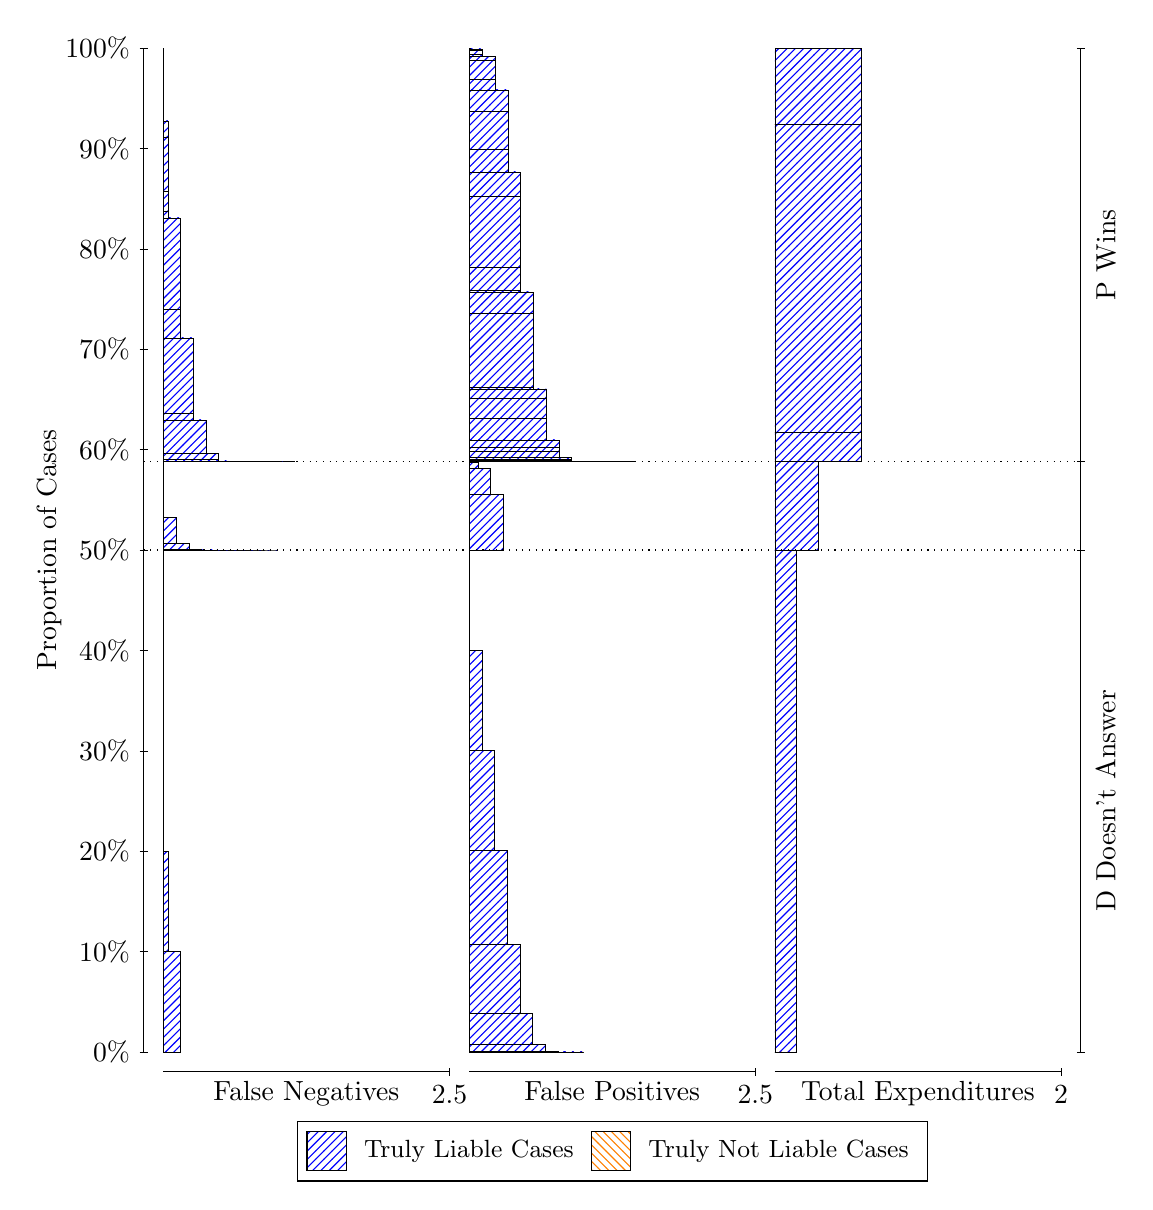
\begin{tikzpicture}
\draw[black, very thin] (1.5,1.75) -- (1.5,14.5);
\node[rotate=90, text=black, anchor=center] at (0.3, 8.125) {Proportion of Cases};
\draw[black, very thin] (1.45,1.75) -- (1.55,1.75);
\node[text=black, anchor=east] at (1.45, 1.75) {0\%};
\draw[black, very thin] (1.45,3.025) -- (1.55,3.025);
\node[text=black, anchor=east] at (1.45, 3.025) {10\%};
\draw[black, very thin] (1.45,4.3) -- (1.55,4.3);
\node[text=black, anchor=east] at (1.45, 4.3) {20\%};
\draw[black, very thin] (1.45,5.575) -- (1.55,5.575);
\node[text=black, anchor=east] at (1.45, 5.575) {30\%};
\draw[black, very thin] (1.45,6.85) -- (1.55,6.85);
\node[text=black, anchor=east] at (1.45, 6.85) {40\%};
\draw[black, very thin] (1.45,8.125) -- (1.55,8.125);
\node[text=black, anchor=east] at (1.45, 8.125) {50\%};
\draw[black, very thin] (1.45,9.4) -- (1.55,9.4);
\node[text=black, anchor=east] at (1.45, 9.4) {60\%};
\draw[black, very thin] (1.45,10.675) -- (1.55,10.675);
\node[text=black, anchor=east] at (1.45, 10.675) {70\%};
\draw[black, very thin] (1.45,11.95) -- (1.55,11.95);
\node[text=black, anchor=east] at (1.45, 11.95) {80\%};
\draw[black, very thin] (1.45,13.225) -- (1.55,13.225);
\node[text=black, anchor=east] at (1.45, 13.225) {90\%};
\draw[black, very thin] (1.45,14.5) -- (1.55,14.5);
\node[text=black, anchor=east] at (1.45, 14.5) {100\%};

\draw[black, very thin] (13.4,1.75) -- (13.4,14.5);
\draw[black, very thin] (13.35,1.75) -- (13.45,1.75);
\node[anchor=west] at (13.35, 1.75) {};
\draw[black, very thin] (13.35,8.125) -- (13.45,8.125);
\node[anchor=west] at (13.35, 8.125) {};
\draw[black, very thin] (13.35,9.2459) -- (13.45,9.2459);
\node[anchor=west] at (13.35, 9.2459) {};
\draw[black, very thin] (13.35,14.5) -- (13.45,14.5);
\node[anchor=west] at (13.35, 14.5) {};

\draw[black, very thin, pattern color=blue, pattern=north east lines] (1.75,1.75) rectangle (1.968,3.025);
\draw[black, very thin, pattern color=blue, pattern=north east lines] (1.75,3.025) rectangle (1.8065,4.2997);
\draw[black, very thin, pattern color=orange, pattern=north west lines] (1.75,4.2997) rectangle (1.75,4.2997);
\draw[black, very thin, pattern color=blue, pattern=north east lines] (1.75,4.2997) rectangle (1.75,8.125);
\draw[black, very thin, pattern color=blue, pattern=north east lines] (1.75,8.125) rectangle (3.2033,8.125);
\draw[black, very thin, pattern color=blue, pattern=north east lines] (1.75,8.125) rectangle (3.0419,8.125);
\draw[black, very thin, pattern color=blue, pattern=north east lines] (1.75,8.125) rectangle (2.8804,8.125);
\draw[black, very thin, pattern color=blue, pattern=north east lines] (1.75,8.125) rectangle (2.7189,8.125);
\draw[black, very thin, pattern color=blue, pattern=north east lines] (1.75,8.125) rectangle (2.5574,8.125);
\draw[black, very thin, pattern color=blue, pattern=north east lines] (1.75,8.125) rectangle (2.3959,8.1252);
\draw[black, very thin, pattern color=blue, pattern=north east lines] (1.75,8.1252) rectangle (2.2344,8.1324);
\draw[black, very thin, pattern color=blue, pattern=north east lines] (1.75,8.1324) rectangle (2.073,8.2096);
\draw[black, very thin, pattern color=blue, pattern=north east lines] (1.75,8.2096) rectangle (1.9115,8.5398);
\draw[black, very thin, pattern color=orange, pattern=north west lines] (1.75,8.5398) rectangle (1.75,8.5398);
\draw[black, very thin, pattern color=blue, pattern=north east lines] (1.75,8.5398) rectangle (1.75,9.2459);
\draw[black, very thin, pattern color=blue, pattern=north east lines] (1.75,9.2459) rectangle (3.4213,9.2459);
\draw[black, very thin, pattern color=blue, pattern=north east lines] (1.75,9.2459) rectangle (3.2599,9.2459);
\draw[black, very thin, pattern color=blue, pattern=north east lines] (1.75,9.2459) rectangle (3.2599,9.2459);
\draw[black, very thin, pattern color=blue, pattern=north east lines] (1.75,9.2459) rectangle (3.0984,9.2459);
\draw[black, very thin, pattern color=blue, pattern=north east lines] (1.75,9.2459) rectangle (3.0984,9.2459);
\draw[black, very thin, pattern color=blue, pattern=north east lines] (1.75,9.2459) rectangle (2.9369,9.2459);
\draw[black, very thin, pattern color=blue, pattern=north east lines] (1.75,9.2459) rectangle (2.7754,9.2464);
\draw[black, very thin, pattern color=blue, pattern=north east lines] (1.75,9.2464) rectangle (2.7754,9.2465);
\draw[black, very thin, pattern color=blue, pattern=north east lines] (1.75,9.2465) rectangle (2.6139,9.2581);
\draw[black, very thin, pattern color=blue, pattern=north east lines] (1.75,9.2581) rectangle (2.4524,9.2734);
\draw[black, very thin, pattern color=blue, pattern=north east lines] (1.75,9.2734) rectangle (2.4524,9.3555);
\draw[black, very thin, pattern color=blue, pattern=north east lines] (1.75,9.3555) rectangle (2.291,9.7785);
\draw[black, very thin, pattern color=blue, pattern=north east lines] (1.75,9.7785) rectangle (2.1295,9.8633);
\draw[black, very thin, pattern color=blue, pattern=north east lines] (1.75,9.8633) rectangle (2.1295,10.819);
\draw[black, very thin, pattern color=blue, pattern=north east lines] (1.75,10.819) rectangle (1.968,11.177);
\draw[black, very thin, pattern color=blue, pattern=north east lines] (1.75,11.177) rectangle (1.968,12.344);
\draw[black, very thin, pattern color=blue, pattern=north east lines] (1.75,12.344) rectangle (1.8065,12.429);
\draw[black, very thin, pattern color=blue, pattern=north east lines] (1.75,12.429) rectangle (1.8065,12.681);
\draw[black, very thin, pattern color=blue, pattern=north east lines] (1.75,12.681) rectangle (1.8065,13.371);
\draw[black, very thin, pattern color=blue, pattern=north east lines] (1.75,13.371) rectangle (1.8065,13.575);
\draw[black, very thin, pattern color=orange, pattern=north west lines] (1.75,13.575) rectangle (1.75,13.575);
\draw[black, very thin, pattern color=blue, pattern=north east lines] (1.75,13.575) rectangle (1.75,14.5);
\draw[black, very thin, pattern color=orange, pattern=north west lines] (5.6333,1.75) rectangle (7.0867,1.75);
\draw[black, very thin, pattern color=blue, pattern=north east lines] (5.6333,1.75) rectangle (7.0867,1.75);
\draw[black, very thin, pattern color=blue, pattern=north east lines] (5.6333,1.75) rectangle (6.9252,1.7503);
\draw[black, very thin, pattern color=blue, pattern=north east lines] (5.6333,1.7503) rectangle (6.7637,1.7583);
\draw[black, very thin, pattern color=blue, pattern=north east lines] (5.6333,1.7583) rectangle (6.6022,1.8435);
\draw[black, very thin, pattern color=blue, pattern=north east lines] (5.6333,1.8435) rectangle (6.4407,2.2369);
\draw[black, very thin, pattern color=blue, pattern=north east lines] (5.6333,2.2369) rectangle (6.2793,3.1185);
\draw[black, very thin, pattern color=blue, pattern=north east lines] (5.6333,3.1185) rectangle (6.1178,4.3083);
\draw[black, very thin, pattern color=blue, pattern=north east lines] (5.6333,4.3083) rectangle (5.9563,5.5753);
\draw[black, very thin, pattern color=blue, pattern=north east lines] (5.6333,5.5753) rectangle (5.7948,6.85);
\draw[black, very thin, pattern color=blue, pattern=north east lines] (5.6333,6.85) rectangle (5.6333,8.125);
\draw[black, very thin, pattern color=orange, pattern=north west lines] (5.6333,8.125) rectangle (6.0693,8.125);
\draw[black, very thin, pattern color=blue, pattern=north east lines] (5.6333,8.125) rectangle (6.0693,8.8311);
\draw[black, very thin, pattern color=blue, pattern=north east lines] (5.6333,8.8311) rectangle (5.9079,9.1613);
\draw[black, very thin, pattern color=blue, pattern=north east lines] (5.6333,9.1613) rectangle (5.7464,9.2385);
\draw[black, very thin, pattern color=blue, pattern=north east lines] (5.6333,9.2385) rectangle (5.6333,9.2459);
\draw[black, very thin, pattern color=orange, pattern=north west lines] (5.6333,9.2459) rectangle (7.7407,9.2459);
\draw[black, very thin, pattern color=blue, pattern=north east lines] (5.6333,9.2459) rectangle (7.7407,9.2459);
\draw[black, very thin, pattern color=orange, pattern=north west lines] (5.6333,9.2459) rectangle (7.5792,9.2459);
\draw[black, very thin, pattern color=blue, pattern=north east lines] (5.6333,9.2459) rectangle (7.5792,9.2459);
\draw[black, very thin, pattern color=orange, pattern=north west lines] (5.6333,9.2459) rectangle (7.4177,9.2459);
\draw[black, very thin, pattern color=blue, pattern=north east lines] (5.6333,9.2459) rectangle (7.4177,9.2459);
\draw[black, very thin, pattern color=blue, pattern=north east lines] (5.6333,9.2459) rectangle (7.4177,9.2459);
\draw[black, very thin, pattern color=orange, pattern=north west lines] (5.6333,9.2459) rectangle (7.2562,9.2459);
\draw[black, very thin, pattern color=blue, pattern=north east lines] (5.6333,9.2459) rectangle (7.2562,9.2464);
\draw[black, very thin, pattern color=orange, pattern=north west lines] (5.6333,9.2464) rectangle (7.0947,9.2464);
\draw[black, very thin, pattern color=blue, pattern=north east lines] (5.6333,9.2464) rectangle (7.0947,9.253);
\draw[black, very thin, pattern color=blue, pattern=north east lines] (5.6333,9.253) rectangle (6.9333,9.2631);
\draw[black, very thin, pattern color=blue, pattern=north east lines] (5.6333,9.2631) rectangle (6.9333,9.2737);
\draw[black, very thin, pattern color=orange, pattern=north west lines] (5.6333,9.2737) rectangle (6.9333,9.2737);
\draw[black, very thin, pattern color=blue, pattern=north east lines] (5.6333,9.2737) rectangle (6.9333,9.3016);
\draw[black, very thin, pattern color=blue, pattern=north east lines] (5.6333,9.3016) rectangle (6.7718,9.3805);
\draw[black, very thin, pattern color=blue, pattern=north east lines] (5.6333,9.3805) rectangle (6.7718,9.4312);
\draw[black, very thin, pattern color=orange, pattern=north west lines] (5.6333,9.4312) rectangle (6.7718,9.4312);
\draw[black, very thin, pattern color=blue, pattern=north east lines] (5.6333,9.4312) rectangle (6.7718,9.5231);
\draw[black, very thin, pattern color=blue, pattern=north east lines] (5.6333,9.5231) rectangle (6.6103,9.797);
\draw[black, very thin, pattern color=orange, pattern=north west lines] (5.6333,9.797) rectangle (6.6103,9.797);
\draw[black, very thin, pattern color=blue, pattern=north east lines] (5.6333,9.797) rectangle (6.6103,10.046);
\draw[black, very thin, pattern color=blue, pattern=north east lines] (5.6333,10.046) rectangle (6.6103,10.17);
\draw[black, very thin, pattern color=blue, pattern=north east lines] (5.6333,10.17) rectangle (6.4488,10.189);
\draw[black, very thin, pattern color=orange, pattern=north west lines] (5.6333,10.189) rectangle (6.4488,10.189);
\draw[black, very thin, pattern color=blue, pattern=north east lines] (5.6333,10.189) rectangle (6.4488,11.136);
\draw[black, very thin, pattern color=blue, pattern=north east lines] (5.6333,11.136) rectangle (6.4488,11.402);
\draw[black, very thin, pattern color=blue, pattern=north east lines] (5.6333,11.402) rectangle (6.2873,11.426);
\draw[black, very thin, pattern color=blue, pattern=north east lines] (5.6333,11.426) rectangle (6.2873,11.719);
\draw[black, very thin, pattern color=orange, pattern=north west lines] (5.6333,11.719) rectangle (6.2873,11.719);
\draw[black, very thin, pattern color=blue, pattern=north east lines] (5.6333,11.719) rectangle (6.2873,12.615);
\draw[black, very thin, pattern color=blue, pattern=north east lines] (5.6333,12.615) rectangle (6.2873,12.926);
\draw[black, very thin, pattern color=blue, pattern=north east lines] (5.6333,12.926) rectangle (6.1259,12.927);
\draw[black, very thin, pattern color=blue, pattern=north east lines] (5.6333,12.927) rectangle (6.1259,13.21);
\draw[black, very thin, pattern color=blue, pattern=north east lines] (5.6333,13.21) rectangle (6.1259,13.698);
\draw[black, very thin, pattern color=blue, pattern=north east lines] (5.6333,13.698) rectangle (6.1259,13.967);
\draw[black, very thin, pattern color=blue, pattern=north east lines] (5.6333,13.967) rectangle (5.9644,13.967);
\draw[black, very thin, pattern color=blue, pattern=north east lines] (5.6333,13.967) rectangle (5.9644,14.1);
\draw[black, very thin, pattern color=blue, pattern=north east lines] (5.6333,14.1) rectangle (5.9644,14.347);
\draw[black, very thin, pattern color=blue, pattern=north east lines] (5.6333,14.347) rectangle (5.9644,14.39);
\draw[black, very thin, pattern color=blue, pattern=north east lines] (5.6333,14.39) rectangle (5.8029,14.424);
\draw[black, very thin, pattern color=blue, pattern=north east lines] (5.6333,14.424) rectangle (5.8029,14.469);
\draw[black, very thin, pattern color=blue, pattern=north east lines] (5.6333,14.469) rectangle (5.8029,14.488);
\draw[black, very thin, pattern color=blue, pattern=north east lines] (5.6333,14.488) rectangle (5.6414,14.499);
\draw[black, very thin, pattern color=blue, pattern=north east lines] (5.6333,14.499) rectangle (5.6414,14.499);
\draw[black, very thin, pattern color=blue, pattern=north east lines] (5.6333,14.499) rectangle (5.6333,14.5);
\draw[black, very thin, pattern color=orange, pattern=north west lines] (9.5167,1.75) rectangle (9.7892,1.75);
\draw[black, very thin, pattern color=blue, pattern=north east lines] (9.5167,1.75) rectangle (9.7892,8.125);
\draw[black, very thin, pattern color=orange, pattern=north west lines] (9.5167,8.125) rectangle (10.062,8.125);
\draw[black, very thin, pattern color=blue, pattern=north east lines] (9.5167,8.125) rectangle (10.062,9.2459);
\draw[black, very thin, pattern color=orange, pattern=north west lines] (9.5167,9.2459) rectangle (10.607,9.2459);
\draw[black, very thin, pattern color=blue, pattern=north east lines] (9.5167,9.2459) rectangle (10.607,9.6178);
\draw[black, very thin, pattern color=orange, pattern=north west lines] (9.5167,9.6178) rectangle (10.607,9.6178);
\draw[black, very thin, pattern color=blue, pattern=north east lines] (9.5167,9.6178) rectangle (10.607,13.533);
\draw[black, very thin, pattern color=orange, pattern=north west lines] (9.5167,13.533) rectangle (10.607,13.533);
\draw[black, very thin, pattern color=blue, pattern=north east lines] (9.5167,13.533) rectangle (10.607,14.5);
\draw[black, dotted] (1.5,8.125) -- (13.4,8.125);
\draw[black, dotted] (1.5,9.2459) -- (13.4,9.2459);
\draw[black, very thin] (1.75,1.5) -- (5.3833,1.5);
\node[text=black, anchor=north] at (3.5667, 1.5) {False Negatives};
\draw[black, very thin] (5.3833,1.45) -- (5.3833,1.55);
\node[text=black, anchor=north] at (5.3833, 1.45) {2.5};

\draw[black, very thin] (5.6333,1.5) -- (9.2667,1.5);
\node[text=black, anchor=north] at (7.45, 1.5) {False Positives};
\draw[black, very thin] (9.2667,1.45) -- (9.2667,1.55);
\node[text=black, anchor=north] at (9.2667, 1.45) {2.5};

\draw[black, very thin] (9.5167,1.5) -- (13.15,1.5);
\node[text=black, anchor=north] at (11.333, 1.5) {Total Expenditures};
\draw[black, very thin] (13.15,1.45) -- (13.15,1.55);
\node[text=black, anchor=north] at (13.15, 1.45) {2};

\node[text=black, centered, rotate=90] at (13.72, 4.9375) {D Doesn't Answer};

\node[text=black, centered, rotate=90] at (13.72, 11.873) {P Wins};

\draw (7.449999999999999,1.5) node[draw=none] (baseCoordinate) {};
\begin{scope}[align=center]
        \matrix[scale=0.5, draw=black, below=0.5cm of baseCoordinate, nodes={draw}, column sep=0.1cm]{
            \node[rectangle, draw, minimum width=0.5cm, minimum height=0.5cm, pattern color=blue, pattern=north east lines] {}; &
            \node[draw=none, font=\small, text=black] (B) {Truly Liable Cases}; &
            \node[rectangle, draw, minimum width=0.5cm, minimum height=0.5cm, pattern color=orange, pattern=north west lines] {}; &
            \node[draw=none, font=\small, text=black] (B) {Truly Not Liable Cases}; \\
            };
\end{scope}

\end{tikzpicture}
\end{document}